% Options for packages loaded elsewhere
\PassOptionsToPackage{unicode}{hyperref}
\PassOptionsToPackage{hyphens}{url}
\documentclass[
]{article}
\usepackage{xcolor}
\usepackage[margin=1in]{geometry}
\usepackage{amsmath,amssymb}
\setcounter{secnumdepth}{-\maxdimen} % remove section numbering
\usepackage{iftex}
\ifPDFTeX
  \usepackage[T1]{fontenc}
  \usepackage[utf8]{inputenc}
  \usepackage{textcomp} % provide euro and other symbols
\else % if luatex or xetex
  \usepackage{unicode-math} % this also loads fontspec
  \defaultfontfeatures{Scale=MatchLowercase}
  \defaultfontfeatures[\rmfamily]{Ligatures=TeX,Scale=1}
\fi
\usepackage{lmodern}
\ifPDFTeX\else
  % xetex/luatex font selection
\fi
% Use upquote if available, for straight quotes in verbatim environments
\IfFileExists{upquote.sty}{\usepackage{upquote}}{}
\IfFileExists{microtype.sty}{% use microtype if available
  \usepackage[]{microtype}
  \UseMicrotypeSet[protrusion]{basicmath} % disable protrusion for tt fonts
}{}
\makeatletter
\@ifundefined{KOMAClassName}{% if non-KOMA class
  \IfFileExists{parskip.sty}{%
    \usepackage{parskip}
  }{% else
    \setlength{\parindent}{0pt}
    \setlength{\parskip}{6pt plus 2pt minus 1pt}}
}{% if KOMA class
  \KOMAoptions{parskip=half}}
\makeatother
\usepackage{color}
\usepackage{fancyvrb}
\newcommand{\VerbBar}{|}
\newcommand{\VERB}{\Verb[commandchars=\\\{\}]}
\DefineVerbatimEnvironment{Highlighting}{Verbatim}{commandchars=\\\{\}}
% Add ',fontsize=\small' for more characters per line
\usepackage{framed}
\definecolor{shadecolor}{RGB}{248,248,248}
\newenvironment{Shaded}{\begin{snugshade}}{\end{snugshade}}
\newcommand{\AlertTok}[1]{\textcolor[rgb]{0.94,0.16,0.16}{#1}}
\newcommand{\AnnotationTok}[1]{\textcolor[rgb]{0.56,0.35,0.01}{\textbf{\textit{#1}}}}
\newcommand{\AttributeTok}[1]{\textcolor[rgb]{0.13,0.29,0.53}{#1}}
\newcommand{\BaseNTok}[1]{\textcolor[rgb]{0.00,0.00,0.81}{#1}}
\newcommand{\BuiltInTok}[1]{#1}
\newcommand{\CharTok}[1]{\textcolor[rgb]{0.31,0.60,0.02}{#1}}
\newcommand{\CommentTok}[1]{\textcolor[rgb]{0.56,0.35,0.01}{\textit{#1}}}
\newcommand{\CommentVarTok}[1]{\textcolor[rgb]{0.56,0.35,0.01}{\textbf{\textit{#1}}}}
\newcommand{\ConstantTok}[1]{\textcolor[rgb]{0.56,0.35,0.01}{#1}}
\newcommand{\ControlFlowTok}[1]{\textcolor[rgb]{0.13,0.29,0.53}{\textbf{#1}}}
\newcommand{\DataTypeTok}[1]{\textcolor[rgb]{0.13,0.29,0.53}{#1}}
\newcommand{\DecValTok}[1]{\textcolor[rgb]{0.00,0.00,0.81}{#1}}
\newcommand{\DocumentationTok}[1]{\textcolor[rgb]{0.56,0.35,0.01}{\textbf{\textit{#1}}}}
\newcommand{\ErrorTok}[1]{\textcolor[rgb]{0.64,0.00,0.00}{\textbf{#1}}}
\newcommand{\ExtensionTok}[1]{#1}
\newcommand{\FloatTok}[1]{\textcolor[rgb]{0.00,0.00,0.81}{#1}}
\newcommand{\FunctionTok}[1]{\textcolor[rgb]{0.13,0.29,0.53}{\textbf{#1}}}
\newcommand{\ImportTok}[1]{#1}
\newcommand{\InformationTok}[1]{\textcolor[rgb]{0.56,0.35,0.01}{\textbf{\textit{#1}}}}
\newcommand{\KeywordTok}[1]{\textcolor[rgb]{0.13,0.29,0.53}{\textbf{#1}}}
\newcommand{\NormalTok}[1]{#1}
\newcommand{\OperatorTok}[1]{\textcolor[rgb]{0.81,0.36,0.00}{\textbf{#1}}}
\newcommand{\OtherTok}[1]{\textcolor[rgb]{0.56,0.35,0.01}{#1}}
\newcommand{\PreprocessorTok}[1]{\textcolor[rgb]{0.56,0.35,0.01}{\textit{#1}}}
\newcommand{\RegionMarkerTok}[1]{#1}
\newcommand{\SpecialCharTok}[1]{\textcolor[rgb]{0.81,0.36,0.00}{\textbf{#1}}}
\newcommand{\SpecialStringTok}[1]{\textcolor[rgb]{0.31,0.60,0.02}{#1}}
\newcommand{\StringTok}[1]{\textcolor[rgb]{0.31,0.60,0.02}{#1}}
\newcommand{\VariableTok}[1]{\textcolor[rgb]{0.00,0.00,0.00}{#1}}
\newcommand{\VerbatimStringTok}[1]{\textcolor[rgb]{0.31,0.60,0.02}{#1}}
\newcommand{\WarningTok}[1]{\textcolor[rgb]{0.56,0.35,0.01}{\textbf{\textit{#1}}}}
\usepackage{longtable,booktabs,array}
\usepackage{calc} % for calculating minipage widths
% Correct order of tables after \paragraph or \subparagraph
\usepackage{etoolbox}
\makeatletter
\patchcmd\longtable{\par}{\if@noskipsec\mbox{}\fi\par}{}{}
\makeatother
% Allow footnotes in longtable head/foot
\IfFileExists{footnotehyper.sty}{\usepackage{footnotehyper}}{\usepackage{footnote}}
\makesavenoteenv{longtable}
\usepackage{graphicx}
\makeatletter
\newsavebox\pandoc@box
\newcommand*\pandocbounded[1]{% scales image to fit in text height/width
  \sbox\pandoc@box{#1}%
  \Gscale@div\@tempa{\textheight}{\dimexpr\ht\pandoc@box+\dp\pandoc@box\relax}%
  \Gscale@div\@tempb{\linewidth}{\wd\pandoc@box}%
  \ifdim\@tempb\p@<\@tempa\p@\let\@tempa\@tempb\fi% select the smaller of both
  \ifdim\@tempa\p@<\p@\scalebox{\@tempa}{\usebox\pandoc@box}%
  \else\usebox{\pandoc@box}%
  \fi%
}
% Set default figure placement to htbp
\def\fps@figure{htbp}
\makeatother
\setlength{\emergencystretch}{3em} % prevent overfull lines
\providecommand{\tightlist}{%
  \setlength{\itemsep}{0pt}\setlength{\parskip}{0pt}}
\usepackage{bookmark}
\IfFileExists{xurl.sty}{\usepackage{xurl}}{} % add URL line breaks if available
\urlstyle{same}
\hypersetup{
  pdftitle={ConRR R Markdown Template},
  pdfauthor={Your Name Here},
  hidelinks,
  pdfcreator={LaTeX via pandoc}}

\title{ConRR R Markdown Template}
\author{Your Name Here}
\date{2025-10-18}

\begin{document}
\maketitle

{
\setcounter{tocdepth}{2}
\tableofcontents
}
\section{Main Heading}\label{main-heading}

This template should help you with the basics of R Markdown: text, code
``chunks'', in-line code, plots and tables. It is easy to make lists,
for example

\begin{itemize}
\tightlist
\item
  Make a list
\item
  Check it twice
\item
  Find out who's naughty and nice
\item
  Come to town
\end{itemize}

Here is some text: just type the same way as you would type in Word.
Directly below this text, there is a code ``chunk'', where you can type
R code:

\begin{Shaded}
\begin{Highlighting}[]
\CommentTok{\# This is a chunk: your R code goes in here just like a regular R script:}
\NormalTok{scores }\OtherTok{\textless{}{-}} \FunctionTok{c}\NormalTok{(}\DecValTok{5}\NormalTok{, }\DecValTok{3}\NormalTok{, }\DecValTok{6}\NormalTok{, }\DecValTok{8}\NormalTok{, }\DecValTok{10}\NormalTok{)}
\NormalTok{m }\OtherTok{\textless{}{-}} \FunctionTok{mean}\NormalTok{(scores)}
\NormalTok{m}
\end{Highlighting}
\end{Shaded}

\begin{verbatim}
## [1] 6.4
\end{verbatim}

\begin{Shaded}
\begin{Highlighting}[]
\NormalTok{pacman}\SpecialCharTok{::}\FunctionTok{p\_load}\NormalTok{(rio, here, ggplot)}
\end{Highlighting}
\end{Shaded}

\begin{verbatim}
## Installing package into 'C:/Users/tekle/AppData/Local/R/win-library/4.5'
## (as 'lib' is unspecified)
\end{verbatim}

\begin{verbatim}
## Warning: package 'ggplot' is not available for this version of R
## 
## A version of this package for your version of R might be available elsewhere,
## see the ideas at
## https://cran.r-project.org/doc/manuals/r-patched/R-admin.html#Installing-packages
\end{verbatim}

\begin{verbatim}
## Warning: unable to access index for repository http://www.stats.ox.ac.uk/pub/RWin/bin/windows/contrib/4.5:
##   cannot open URL 'http://www.stats.ox.ac.uk/pub/RWin/bin/windows/contrib/4.5/PACKAGES'
\end{verbatim}

\begin{verbatim}
## Warning in p_install(package, character.only = TRUE, ...):
\end{verbatim}

\begin{verbatim}
## Warning in library(package, lib.loc = lib.loc, character.only = TRUE,
## logical.return = TRUE, : there is no package called 'ggplot'
\end{verbatim}

\begin{verbatim}
## Warning in pacman::p_load(rio, here, ggplot): Failed to install/load:
## ggplot
\end{verbatim}

\begin{Shaded}
\begin{Highlighting}[]
\NormalTok{films }\OtherTok{\textless{}{-}} \FunctionTok{import}\NormalTok{(}\FunctionTok{here}\NormalTok{(}\StringTok{\textquotesingle{}1\_data/films.csv\textquotesingle{}}\NormalTok{)) }

\FunctionTok{head}\NormalTok{(films)}
\end{Highlighting}
\end{Shaded}

\begin{verbatim}
##   V1    tconst averageRating numVotes titleType              primaryTitle
## 1  1 tt0252994           8.0       16     short   Climbing Jacob's Ladder
## 2  2 tt2369678           6.0        9   tvMovie In Sickness and in Health
## 3  3 tt0069282           6.2     1023     movie                   Slither
## 4  4 tt1861338           8.2        8     short       God Bless the Child
## 5  5 tt0821815           6.6       16   tvMovie              Westward Ho!
## 6  6 tt0047180           7.7      424     movie                  Liliomfi
##               originalTitle startYear endYear runtimeMinutes
## 1   Climbing Jacob's Ladder      1899     \\N            \\N
## 2 In Sickness and in Health      2012     \\N             88
## 3                   Slither      1973     \\N             97
## 4       God Bless the Child      2011     \\N              3
## 5              Westward Ho!      1988     \\N             55
## 6                  Liliomfi      1955     \\N            109
##                       genres
## 1          Documentary,Short
## 2                     Family
## 3      Comedy,Crime,Thriller
## 4               Comedy,Short
## 5 Adventure,Animation,Comedy
## 6                     Comedy
\end{verbatim}

\begin{Shaded}
\begin{Highlighting}[]
\NormalTok{ave.vot}\OtherTok{\textless{}{-}} \FunctionTok{ggplot}\NormalTok{(}\AttributeTok{data =}\NormalTok{ films, }\AttributeTok{mapping =} \FunctionTok{aes}\NormalTok{(}\AttributeTok{x =}\NormalTok{ averageRating, }\AttributeTok{y =}\NormalTok{ numVotes))}\SpecialCharTok{+}
  \FunctionTok{geom\_point}\NormalTok{()}\SpecialCharTok{+}
  \FunctionTok{labs}\NormalTok{(}\AttributeTok{title =} \StringTok{\textquotesingle{}Relationship between the number of votes and average rate of the films\textquotesingle{}}\NormalTok{,}
       \AttributeTok{x =} \StringTok{\textquotesingle{}Average Rating\textquotesingle{}}\NormalTok{,}
       \AttributeTok{y =} \StringTok{\textquotesingle{}Number of votes\textquotesingle{}}\NormalTok{,}
       \AttributeTok{caption =} \StringTok{\textquotesingle{}Source: Films data set\textquotesingle{}}\NormalTok{)}
\end{Highlighting}
\end{Shaded}

\subsection{Sub-heading: chunk options}\label{sub-heading-chunk-options}

By default, knitr will show both your code and the output in the
resulting document. You can use chunk options to change this behaviour.
They work like R command arguments. First, tell knitr to not show the
code, by using \texttt{echo=FALSE}:

\begin{verbatim}
## [1] 6.4
\end{verbatim}

Second, tell knitr to not show the output, using
\texttt{results=\textquotesingle{}hide}:

\begin{Shaded}
\begin{Highlighting}[]
\NormalTok{scores }\OtherTok{\textless{}{-}} \FunctionTok{c}\NormalTok{(}\DecValTok{5}\NormalTok{, }\DecValTok{3}\NormalTok{, }\DecValTok{6}\NormalTok{, }\DecValTok{8}\NormalTok{, }\DecValTok{10}\NormalTok{)}
\NormalTok{the.mean }\OtherTok{\textless{}{-}} \FunctionTok{mean}\NormalTok{(scores)}
\NormalTok{the.mean}
\end{Highlighting}
\end{Shaded}

You can also tell knitr to not run the code at all, using
\texttt{eval=FALSE}:

\begin{Shaded}
\begin{Highlighting}[]
\NormalTok{scores10 }\OtherTok{\textless{}{-}} \FunctionTok{c}\NormalTok{(}\DecValTok{5}\NormalTok{, }\DecValTok{3}\NormalTok{, }\DecValTok{6}\NormalTok{, }\DecValTok{8}\NormalTok{, }\DecValTok{10}\NormalTok{, }\DecValTok{3}\NormalTok{, }\DecValTok{6}\NormalTok{, }\DecValTok{12}\NormalTok{, }\DecValTok{4}\NormalTok{, }\DecValTok{9}\NormalTok{)}
\FunctionTok{mean}\NormalTok{(scores10)}
\end{Highlighting}
\end{Shaded}

Instead of setting these options in every chunk, you can set options at
the beginning that will then be in place for every chunk. We call this a
``global'' chunk option, and we do this in the very first chunk in this
document where we set \texttt{echo=TRUE} using the line
\texttt{knitr::opts\_chunk\$set(echo\ =\ TRUE)}.

A useful aspect of R Markdown is that, in the text, you can use objects
that you've created inside the chunks. For example, the mean of
\texttt{scores} is 6.4. You can even run little bits of code inside the
text: the sum of the five scores is 32, for example.

\subsection{Sub-heading: plots}\label{sub-heading-plots}

You can run code that creates plots, and knitr will show them by
default:

\begin{Shaded}
\begin{Highlighting}[]
\NormalTok{myplot }\OtherTok{\textless{}{-}} \FunctionTok{ggplot}\NormalTok{(}\AttributeTok{data=}\NormalTok{diamonds, }\FunctionTok{aes}\NormalTok{(}\AttributeTok{x=}\NormalTok{cut, }\AttributeTok{y=}\NormalTok{price, }\AttributeTok{fill=}\NormalTok{color)) }\SpecialCharTok{+}
  \FunctionTok{geom\_bar}\NormalTok{(}\AttributeTok{stat=}\StringTok{"identity"}\NormalTok{)}\SpecialCharTok{+}
  \FunctionTok{scale\_fill\_brewer}\NormalTok{(}\AttributeTok{palette=}\StringTok{"Set3"}\NormalTok{)}
\NormalTok{myplot}
\end{Highlighting}
\end{Shaded}

\pandocbounded{\includegraphics[keepaspectratio]{index_files/figure-latex/unnamed-chunk-4-1.pdf}}

\subsubsection{Sub-sub-heading: chunk options for
plots}\label{sub-sub-heading-chunk-options-for-plots}

There are also chunk options that let you alter your plot, such as
specifying the dimensions:

\pandocbounded{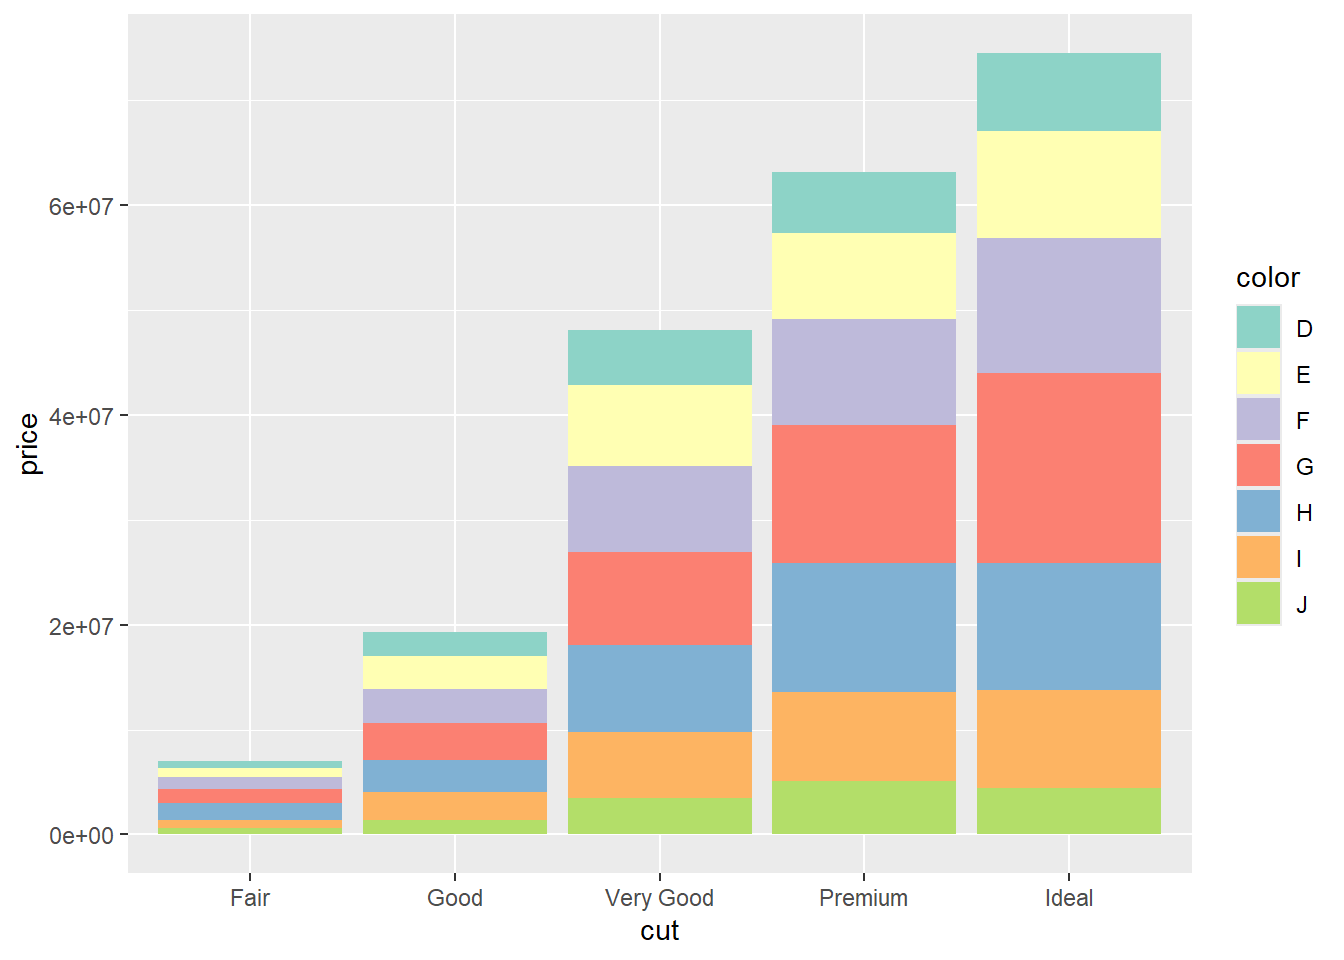
\includegraphics[keepaspectratio]{index_files/figure-latex/unnamed-chunk-5-1.pdf}}

\subsection{Tables}\label{tables}

\subsubsection{kable: for basic tables}\label{kable-for-basic-tables}

The \texttt{kable} command is a fast way to create tables. Here is the
simple output of R without using any commands:

\begin{Shaded}
\begin{Highlighting}[]
\NormalTok{tab }\OtherTok{\textless{}{-}} \FunctionTok{head}\NormalTok{(diamonds[, }\DecValTok{1}\SpecialCharTok{:}\DecValTok{7}\NormalTok{])}
\NormalTok{tab}
\end{Highlighting}
\end{Shaded}

\begin{verbatim}
## # A tibble: 6 x 7
##   carat cut       color clarity depth table price
##   <dbl> <ord>     <ord> <ord>   <dbl> <dbl> <int>
## 1  0.23 Ideal     E     SI2      61.5    55   326
## 2  0.21 Premium   E     SI1      59.8    61   326
## 3  0.23 Good      E     VS1      56.9    65   327
## 4  0.29 Premium   I     VS2      62.4    58   334
## 5  0.31 Good      J     SI2      63.3    58   335
## 6  0.24 Very Good J     VVS2     62.8    57   336
\end{verbatim}

Now using \texttt{kable}:

\begin{Shaded}
\begin{Highlighting}[]
\FunctionTok{kable}\NormalTok{(tab)}
\end{Highlighting}
\end{Shaded}

\begin{longtable}[]{@{}rlllrrr@{}}
\toprule\noalign{}
carat & cut & color & clarity & depth & table & price \\
\midrule\noalign{}
\endhead
\bottomrule\noalign{}
\endlastfoot
0.23 & Ideal & E & SI2 & 61.5 & 55 & 326 \\
0.21 & Premium & E & SI1 & 59.8 & 61 & 326 \\
0.23 & Good & E & VS1 & 56.9 & 65 & 327 \\
0.29 & Premium & I & VS2 & 62.4 & 58 & 334 \\
0.31 & Good & J & SI2 & 63.3 & 58 & 335 \\
0.24 & Very Good & J & VVS2 & 62.8 & 57 & 336 \\
\end{longtable}

The \texttt{kable} command has arguments for altering how the table
looks, including changing the column names, alignment, captions,
rounding, and more.

\begin{Shaded}
\begin{Highlighting}[]
\NormalTok{better.colnames }\OtherTok{\textless{}{-}} \FunctionTok{c}\NormalTok{(}\StringTok{"Carat"}\NormalTok{, }\StringTok{"Cut"}\NormalTok{, }\StringTok{"Colour"}\NormalTok{, }\StringTok{"Clarity"}\NormalTok{, }\StringTok{"Depth(\%)"}\NormalTok{, }\StringTok{"Relative width"}\NormalTok{, }\StringTok{"Price($)"}\NormalTok{)}
\NormalTok{better.tab }\OtherTok{\textless{}{-}} \FunctionTok{kable}\NormalTok{(tab,}
      \AttributeTok{col.names =}\NormalTok{ better.colnames,}
      \AttributeTok{align =} \FunctionTok{c}\NormalTok{(}\StringTok{"rcccrrr"}\NormalTok{),}
      \AttributeTok{caption =} \StringTok{"My sensible caption"}\NormalTok{)}
\NormalTok{better.tab}
\end{Highlighting}
\end{Shaded}

\begin{longtable}[]{@{}
  >{\raggedleft\arraybackslash}p{(\linewidth - 12\tabcolsep) * \real{0.0896}}
  >{\centering\arraybackslash}p{(\linewidth - 12\tabcolsep) * \real{0.1642}}
  >{\centering\arraybackslash}p{(\linewidth - 12\tabcolsep) * \real{0.1194}}
  >{\centering\arraybackslash}p{(\linewidth - 12\tabcolsep) * \real{0.1343}}
  >{\raggedleft\arraybackslash}p{(\linewidth - 12\tabcolsep) * \real{0.1343}}
  >{\raggedleft\arraybackslash}p{(\linewidth - 12\tabcolsep) * \real{0.2239}}
  >{\raggedleft\arraybackslash}p{(\linewidth - 12\tabcolsep) * \real{0.1343}}@{}}
\caption{My sensible caption}\tabularnewline
\toprule\noalign{}
\begin{minipage}[b]{\linewidth}\raggedleft
Carat
\end{minipage} & \begin{minipage}[b]{\linewidth}\centering
Cut
\end{minipage} & \begin{minipage}[b]{\linewidth}\centering
Colour
\end{minipage} & \begin{minipage}[b]{\linewidth}\centering
Clarity
\end{minipage} & \begin{minipage}[b]{\linewidth}\raggedleft
Depth(\%)
\end{minipage} & \begin{minipage}[b]{\linewidth}\raggedleft
Relative width
\end{minipage} & \begin{minipage}[b]{\linewidth}\raggedleft
Price(\$)
\end{minipage} \\
\midrule\noalign{}
\endfirsthead
\toprule\noalign{}
\begin{minipage}[b]{\linewidth}\raggedleft
Carat
\end{minipage} & \begin{minipage}[b]{\linewidth}\centering
Cut
\end{minipage} & \begin{minipage}[b]{\linewidth}\centering
Colour
\end{minipage} & \begin{minipage}[b]{\linewidth}\centering
Clarity
\end{minipage} & \begin{minipage}[b]{\linewidth}\raggedleft
Depth(\%)
\end{minipage} & \begin{minipage}[b]{\linewidth}\raggedleft
Relative width
\end{minipage} & \begin{minipage}[b]{\linewidth}\raggedleft
Price(\$)
\end{minipage} \\
\midrule\noalign{}
\endhead
\bottomrule\noalign{}
\endlastfoot
0.23 & Ideal & E & SI2 & 61.5 & 55 & 326 \\
0.21 & Premium & E & SI1 & 59.8 & 61 & 326 \\
0.23 & Good & E & VS1 & 56.9 & 65 & 327 \\
0.29 & Premium & I & VS2 & 62.4 & 58 & 334 \\
0.31 & Good & J & SI2 & 63.3 & 58 & 335 \\
0.24 & Very Good & J & VVS2 & 62.8 & 57 & 336 \\
\end{longtable}

More details on \texttt{kable} here:
\url{https://bookdown.org/yihui/rmarkdown-cookbook/kable.html}

\end{document}
